\section{تعيين المحاور الإحداثية (\LR{Coordinate Frames Assignment})}
\label{sec:frames}

الخطوة الأولى في خوارزمية دينافيت-هارتنبيرغ (\LR{DH}) هي ربط جملة إحداثيات ديكارتية محلية بكل وصلة من وصلات الروبوت، بدءاً من القاعدة الثابتة (\LR{Base}) وصولاً إلى المؤثر النهائي. بالنسبة للروبوت (\LR{SCARA}) المدروس، تم توجيه المحاور وفق القواعد الهندسية التالية:

 \begin{figure}[H]
     \centering
     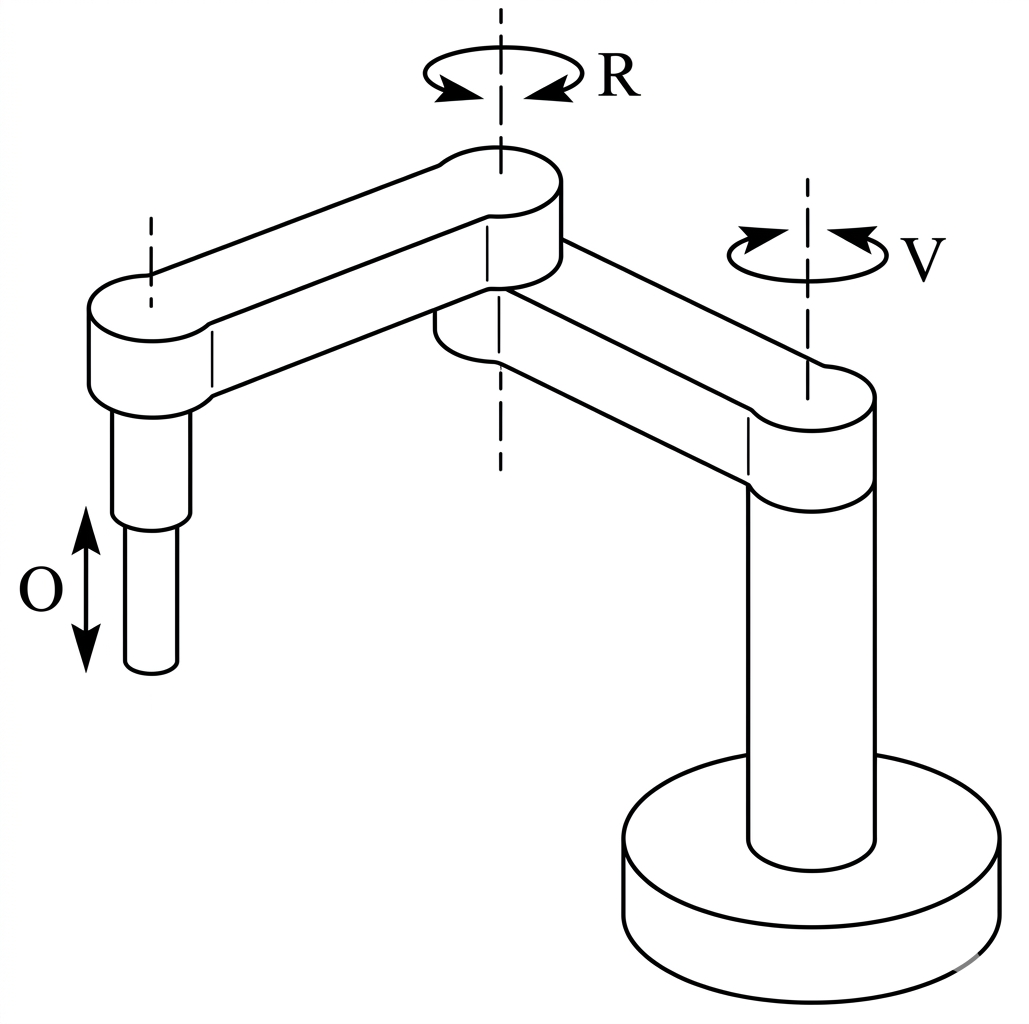
\includegraphics[width=0.7\textwidth]{resources/images/scara_arm}
%     \caption{توزيع المحاور الإحداثية على مفاصل الروبوت وفق خوارزمية \LR{DH}}
     \label{fig:frames}
 \end{figure}

\begin{itemize}
    \item \textbf{المحاور $Z_0$ و $Z_1$:} تم توجيهها عمودياً على المستوي الأفقي لتمثل محاور الدوران للمفصلين الأول والثاني.
    \item \textbf{المحور $Z_2$:} يمثل محور الحركة الانسحابية للمفصل الثالث، وتم توجيهه نحو الأسفل (باتجاه منطقة العمل).
    \item \textbf{المحاور $X_i$:} تم توجيهها على امتداد الوصلات الميكانيكية (\LR{Links}) بحيث تكون عمودية على المحور $Z_{i-1}$ وتتقاطع معه.
\end{itemize}

